% ------------------------------------------------------------------------------------
\newpage
\section{Ejercicio 2}
\textbf{(Estudio de mercado)} Se tiene un producto y se realiza una encuesta con el fin de estudiar cuánto se consume dependiendo de la edad. Sea $Y_{i}$ el monto de compra y $X_{i}$ la covariable la cual representa la edad.
	
Suponga que $Y_{i} \sim Po \left(\lambda_{i}\right)$ (distribución Poisson con intensidad $ \lambda_{i}$)
\begin{equation} \label{eq:15}
	\lambda_{i}=c g_{b}\left(x_{i}-a\right)
\end{equation}
para $g_{b}$ la siguiente función de liga
\begin{equation} \label{eq:16}
	g_{b}(x)=\exp \left(-\frac{x^{2}}{2 b^{2}}\right).
\end{equation}
O sea, se trata de regresión Poisson con una función liga no usual. Si $\lambda_{i}=0$ entonces $P \left(Y_{i}=0\right) = 1$. $a=$ años medio del segmento (años), $c =$ gasto promedio (pesos), $b=$ "amplitud" del segmento (años).
	
Considere las distribuciones a priori
\begin{equation} \label{eq:17}
	a \sim N(35,5), \quad c \sim Gama (3,3 / 950), \quad b \sim Gama (2,2 / 5).
\end{equation}
El segundo parámetro de la normal es desviación estandard y el segundo parámetro de las gammas es tasa (\textit{rate}).
	
Usando MH simule de la distribución posterior de $a$, $c$ y $b$.
	
Los datos son estos, $n = 100$ :
	
\begin{figure}[h!]
	\centering
	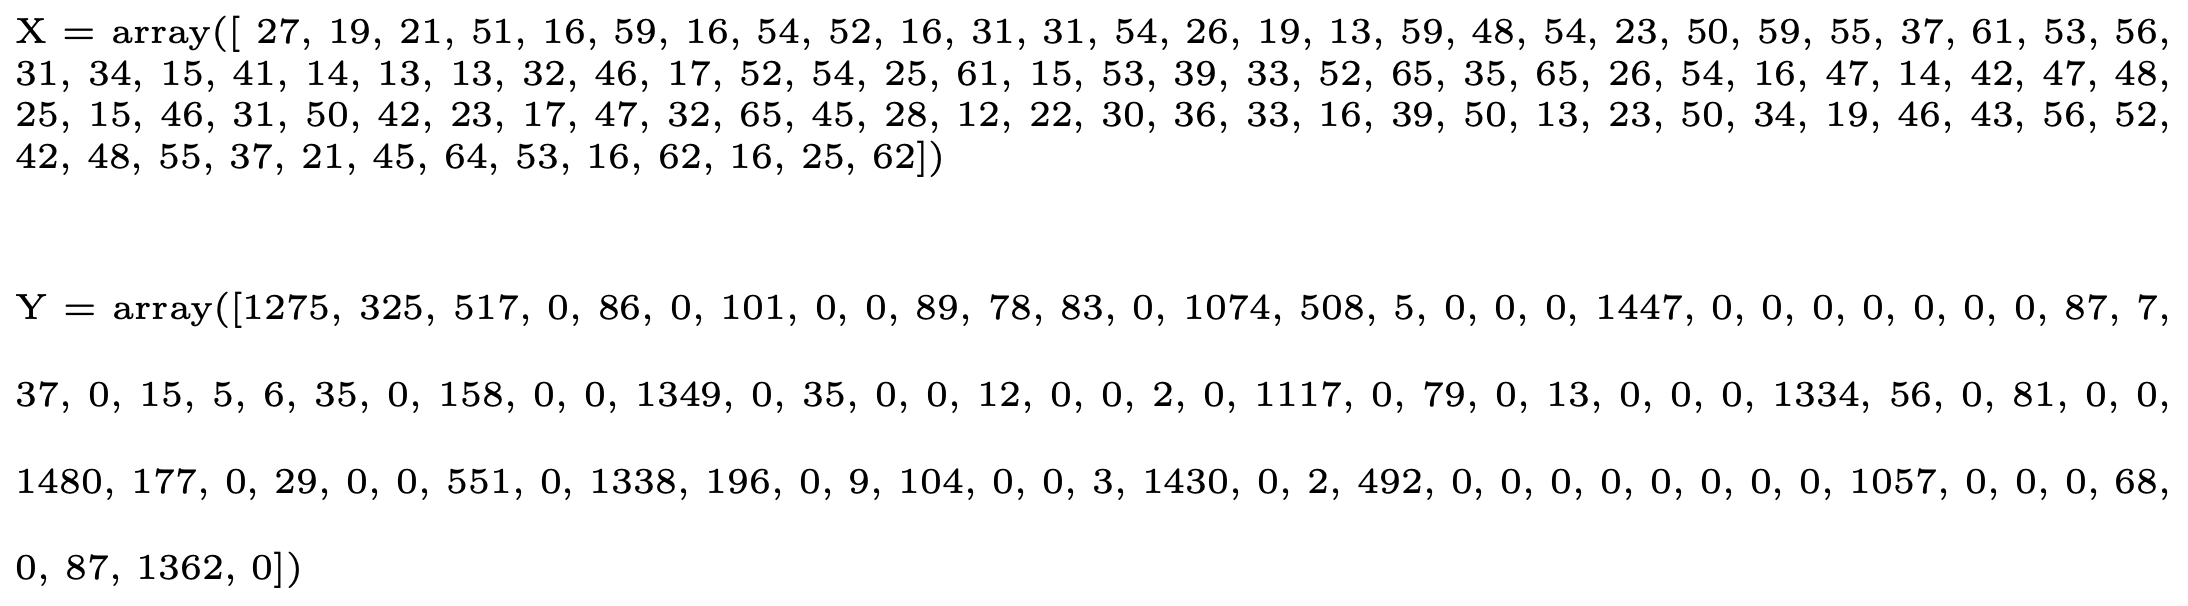
\includegraphics[width=\textwidth]{IMAGENES/captura}
\end{figure}
	
\vspace{5mm}
{\color{gray} \hrule}
\vspace{5mm}
\textcolor{BrickRed}{\it Respuesta:}

Se tiene que $\lambda_{i} := \lambda_{i}(a,b,c) = c\cdot e^{- \frac{(x_i -a)^2}{2b^2}}$ y se quiere hacer inferencia sobre $a$, $b$ y $c$. Como $Y_i\sim Po(\lambda_{i})$, entonces
\begin{equation} \label{eq:18}
	P(Y_i = y_i \mid \lambda_{i} (a,b,c)) = \frac{\lambda_{i}^{y_i} e^{-\lambda_{i}}}{y_i !}
\end{equation}
Entonces, la probabilidad conjunta para $n$ observaciones $Y=\{Y_{1}, \dots, Y_{n}\}$ suponiendo independencia condicional dada $\lambda = \{\lambda_{1}, \dots, \lambda_{n}\}$ es:
\begin{equation}\label{eq:19}
	P(Y = y \mid a,b,c) = \prod_{i=1}^{n} \frac{\lambda_{i}^{y_i} e^{-\lambda_{i}}}{y_i !}
\end{equation}
para $y=\{y_{1}, \dots, y_{n}\}$. La ecuación \eqref{eq:19} es la verosimilitud y de la expresión \eqref{eq:17}, se tiene las distribuciones a priori, esto da lugar a la posterior
\begin{equation} \label{eq:20}
	\begin{aligned}
		P(a,b,c &\mid Y = y)
		\propto P(Y = y \mid a,b,c) \cdot \pi_{a} \left(a\right) \cdot \pi_{b} \left(b\right) \cdot \pi_{c} \left(c\right) \cdot \mathbbm{1}_{\mathbb{R}} (a) \mathbbm{1}_{(0,\infty)} (b) \mathbbm{1}_{(0,\infty)} (c)\\
		&\propto \prod_{i=1}^{n} \frac{\lambda_{i}^{y_i} e^{-\lambda_{i}}}{y_i !}
		\cdot \frac{1}{5\cdot \sqrt{2\pi}} e^{-\frac{(a - 35)^2}{2 \cdot 5^2}} \cdot  \frac{(2/5)^2}{\Gamma(2)} b^{2-1} e^{-b \cdot (2/5)} \cdot  \frac{(3/950)^3}{\Gamma(3)} c^{3-1} e^{-c \cdot (3/950)} \\
		&\propto bc^{2} e^{-\frac{(a - 35)^2}{50}} e^{-\frac{2}{5}b} e^{-\frac{3}{950}c} \cdot \prod_{i=1}^{n} \lambda_{i}^{y_i} e^{-\lambda_{i}} \cdot \mathbbm{1}_{\mathbb{R}} (a) \mathbbm{1}_{(0,\infty)} (b) \mathbbm{1}_{(0,\infty)} (c)\\
		& \propto bc^{2} e^{-\frac{(a - 35)^2}{50}} e^{-\frac{2}{5}b} e^{-\frac{3}{950}c} \cdot e^{-\sum \lambda_{i}} \prod_{i=1}^{n} \left( c e^{- \frac{(x_i -a)^2}{2b^2}} \right)^{y_i}  \cdot \mathbbm{1}_{\mathbb{R}} (a) \mathbbm{1}_{(0,\infty)} (b) \mathbbm{1}_{(0,\infty)} (c)\\
		& \propto bc^{2} e^{-\frac{(a - 35)^2}{50}} e^{-\frac{2}{5}b} e^{-\frac{3}{950}c} \cdot e^{-c\sum e^{- \frac{(x_i -a)^2}{2b^2}}} c^{\sum y_i} \cdot \prod_{i=1}^{n} e^{- y_i\frac{(x_i -a)^2}{2b^2}} \cdot \mathbbm{1}_{\mathbb{R}} (a) \mathbbm{1}_{(0,\infty)} (b) \mathbbm{1}_{(0,\infty)} (c)\\
		& \propto c^{2 + \sum y_i} e^{-c \left(\frac{3}{950} + \sum e^{- \frac{(x_i -a)^2}{2b^2}}\right)} \cdot b e^{-\frac{(a - 35)^2}{50}} e^{-\frac{2}{5}b} e^{- \sum y_i\frac{(x_i -a)^2}{2b^2}} \cdot \mathbbm{1}_{\mathbb{R}} (a) \mathbbm{1}_{(0,\infty)} (b) \mathbbm{1}_{(0,\infty)} (c)
	\end{aligned}
\end{equation}
Esta expresión nos sirve para encontrar una propuesta Gibbs para el algoritmo de Metropolis Hastings con kérneles híbridos. Se puede notar que no existe una forma cerrada estándar para ninguna de las condicionales completas para $a$ y $b$ para muestrear directamente debido a la complejidad del producto de la derecha. Sin embargo, nótese que el término
\begin{equation} \label{eq:21}
	c^{2 + \sum y_i} e^{-c \left(\frac{3}{950} + \sum e^{- \frac{(x_i -a)^2}{2b^2}}\right)}
\end{equation}
es proporcional a una distribución
\begin{equation} \label{eq:22}
	Gama\left(3+\sum y_i, \frac{3}{950} + \sum e^{- \frac{(x_i -a)^2}{2b^2}}\right)
\end{equation}
para $c$ dados $a$, $b$ y los datos, la cual se puede usar como una propuesta Gibbs. En el archivo \textcolor{mediumblue}{ejercicio2\_tarea9.py} se hace uso de la función:
\begin{center}
	\textit{METROPOLIS\_HASTINGS\_HYBRID\_KERNELS()},
\end{center}
implementada en el archivo \textcolor{mediumblue}{ejercicio1\_tarea9.py} e importada al actual, la cual aplica el algoritmo Metropolis-Hastings con kérneles híbridos para $K$ propuestas simulando una cadena de Markov en $\mathbb{R}^n$. Se comienza definiendo las funciones \eqref{eq:15} y \eqref{eq:16} que son necesarias para la función \textit{posterior()} la cual implementa la función objetivo descrita en \eqref{eq:20}

\textbf{Distribución inicial:}

Por simplicidad y  buenos resultados al momento de experimentar con las distintas propuestas y distribuciones iniciales, se decidió usar como distribución inicial las a prioris \eqref{eq:17}:
\begin{equation} \label{eq:23}
		a \sim N(35,5), \quad c \sim Gama (3,3 / 950), \quad b \sim Gama (2,2 / 5).
\end{equation}

\textbf{Propuestas:}

En el archivo \textcolor{mediumblue}{ejercicio1\_tarea9.py}, se implementan las propuestas, así como su densidad de probabilidad respectiva y estas se describen a continuación.

\begin{itemize}
	\item \underline{Propuesta 1:} 	Kérnel Gibbs para $c$ dados $a$, $b$ y los datos.
	\begin{equation} \label{eq:24}
		c\sim Gama\left(3+\sum y_i, \frac{3}{950} + \sum e^{- \frac{(x_i -a)^2}{2b^2}}\right) \text{ y } a, b \text{ fijos.}
	\end{equation}
\end{itemize}
Se define la función \textit{prop\_gibbs\_c\_gen()} que implementa la distribución Gibbs (distribución condicional de $c$ dado $a$, $b$) descrita en \eqref{eq:22}. También se define su densidad de probabilidad en la función \textit{prop\_gibbs\_c\_pdf()}. Se eligió esta propuesta ya que un paso de Gibbs siempre acepta la propuesta porque la muestra proviene de la distribución condicional verdadera. Esto asegura exploración eficiente en la dimensión de $c$, además de más detalles descritos en la parte de conclusiones.

\begin{itemize}
	\item \underline{Propuesta 2:} 	Caminata aleatoria conjunta.
	\begin{equation} \label{eq:25}
		a_p\sim \mathcal{N} (a, \sigma_a),\quad b_p\sim \mathcal{N} (b, \sigma_b),\quad c_p\sim \mathcal{N} (c, \sigma_c)
	\end{equation}
\end{itemize}
Se decidió usar esta propuesta ya que en cadenas de Markov, son robustas para exploración local y garantizan una tasa de aceptación razonable. Sin embargo, su convergencia puede ser lenta si la posterior es amplia, pero para ese caso, ya se cuentan con otras propuestas que cuentan con más variabilidad. Para cada parámetro, se eligió su varianza $\sigma$, experimentando y revisando los soportes de cada parámetro, así como de su desempeño en la mayoría de los experimentos, se eligió usar $\sigma_a = 5$, $\sigma_b = 5/2$ y $\sigma_a = 950/3$ (también para usar parámetros ya definidos en otras distribuciones). La función generadora y su función de densidad se definen en \textit{prop\_normal\_conjunta\_gen()} y \textit{prop\_normal\_conjunta\_pdf()} respectivamente.

\begin{itemize}
	\item \underline{Propuesta 3 y 4:} Propuestas a priori.
	\begin{equation} \label{eq:26}
		\begin{aligned}
			&a\sim \mathcal{N}(35,5) \text{ y } b, c \text{ fijos},\\
			&b\sim Gama(3, 2/5) \text{ y } a, c \text{ fijos}.
		\end{aligned}
	\end{equation}
\end{itemize}
Se eligieron estas propuestas, ya que, dado que son propuestas independientes para sus respectivos parámetros, introducen aleatoriedad independiente de los datos, lo que ayuda a evitar que la cadena quede atrapada en un modo local y permite exploración de regiones remotas del espacio de parámetros. Las funciones que las describen son
\begin{itemize}
	\item \textit{prop\_a\_apriori\_gen()} y \textit{prop\_a\_apriori\_gen()}
	\item \textit{prop\_b\_apriori\_gen()} y \textit{prop\_b\_apriori\_gen()}
\end{itemize}
Se eligió no usar la a priori de $c$ ya que presentaba más variabilidad y dado que ya se tiene una Gibbs, se observó un mejor desempeño que cuando se mezclaban ambas.

\textbf{Conclusión general de las propuestas:}

Para garantizar una buena convergencia, las elecciones de las propuestas aprovechan tanto la estructura condicional de la posterior como las propiedades específicas de cada parámetro. La elección de la propuesta Gibbs siempre es óptima porque utiliza la condicional completa de $c$. Esto garantiza aceptación total y evita rechazos, maximizando la eficiencia del muestreo. Su capacidad de incorporar la interacción de $c$ con los datos y otros parámetros la hace ideal para una convergencia rápida, esto se ve evidente en los resultados mostrados a continuación

Las propuestas prior para $a$ y $b$ resultan ser una buena elección, ya que respeta la información a priori y permite explorar eficientemente la región inicial del espacio de parámetros. Las propuestas basadas en las distribuciones a priori garantizan que la cadena comience en regiones razonables, evitando problemas de inicialización. La propuesta normal conjunta para $a$, $b$, y $c$ resultó interesante ya que generar propuestas conjuntas permite capturar dependencias que podrían pasar desapercibidas con propuestas independientes.

En conjunto, esta estrategia híbrida combina la precisión y eficiencia del Gibbs Sampling con la flexibilidad de propuestas adaptativas, asegurando convergencia rápida y una buena exploración del espacio posterior.

\textbf{Resultados:}

Nuevamente, con  ayuda de las funciones auxiliares descritas en \ref{sec:funauc} e implementadas en \textcolor{mediumblue}{funciones\_auxiliares.py}, se puede visualizar los resultados generados. Se ejecuta el código principal, en el cual se definen los datos a tratar, así como los parámetros para la distribución posterior, las a priori, la inicial y las propuestas. Para el algoritmo Metropolis-Hastings sólo fueron necesarias $2000$ muestras ya que, en distintos experimentos se vio que la cadena cae en estados estacionarios, algunos temporales y otros permanentes. En este caso, se quedó en el estado estacionario final bastante pronto.

El punto inicial resultó ser $[34.6139, 9.5969, 839.8066]$ (se usó una semilla para la reproducibilidad de los resultados). A continuación, se definieron las listas de funciones generadoras de cada propuesta, así como de sus respectivas funciones de densidad y a todas las propuestas se les dio probabilidad de elección igual a $\frac{1}{4}$. Al generar la cadena, se obtuvo un $41.45\%$ de aceptación de propuestas y con ayuda de la función \textit{estim\_burn\_in\_and\_modes()} se calcularon las modas resultantes de cada parámetro y el burn-in a considerar: moda de $a$: $23.653$, moda de $b$: $3.143$, moda de $c$: $1498.342$ y el burn-in: $349$. Los valores resultantes de estas modas fueron bastante recurrentes para distintos puntos iniciales y configuraciones de las propuestas. A continuación se tienen los histogramas de las cadenas de Markov simuladas.
\begin{figure}[h!]
	\centering
	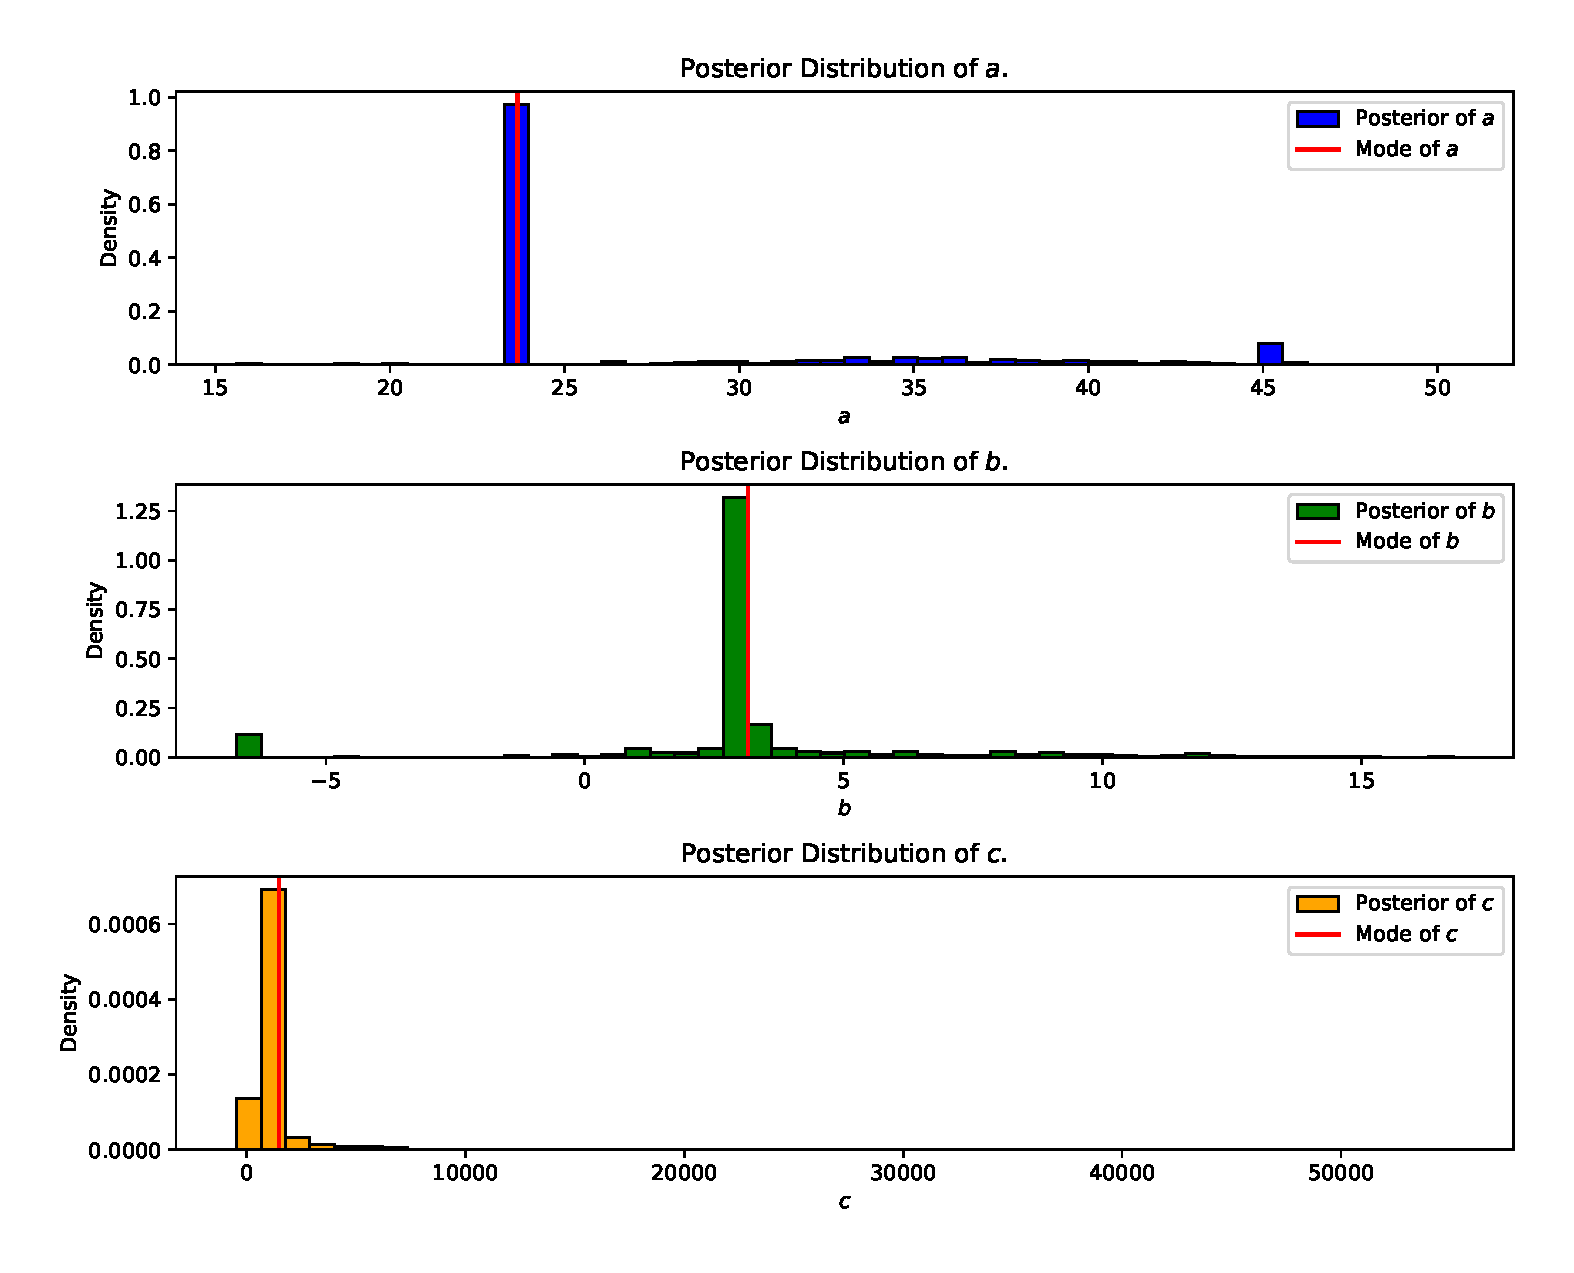
\includegraphics[width=0.845\textwidth]{IMAGENES/histogram_ex2.pdf}
\end{figure}

A continuación, se tiene la evolución de las cadenas de Markov marginales con respecto al burn-in estimado. Podemos notar que al principio, la cadena cayó en un estado estacionario temporal, es por eso que el burn-in se tomó en esta zona y la razón por la que se eligió mostrar este ejemplo particular ya que fenómenos como este sucedieron en cada experimento.

\begin{figure}[h!]
	\centering
	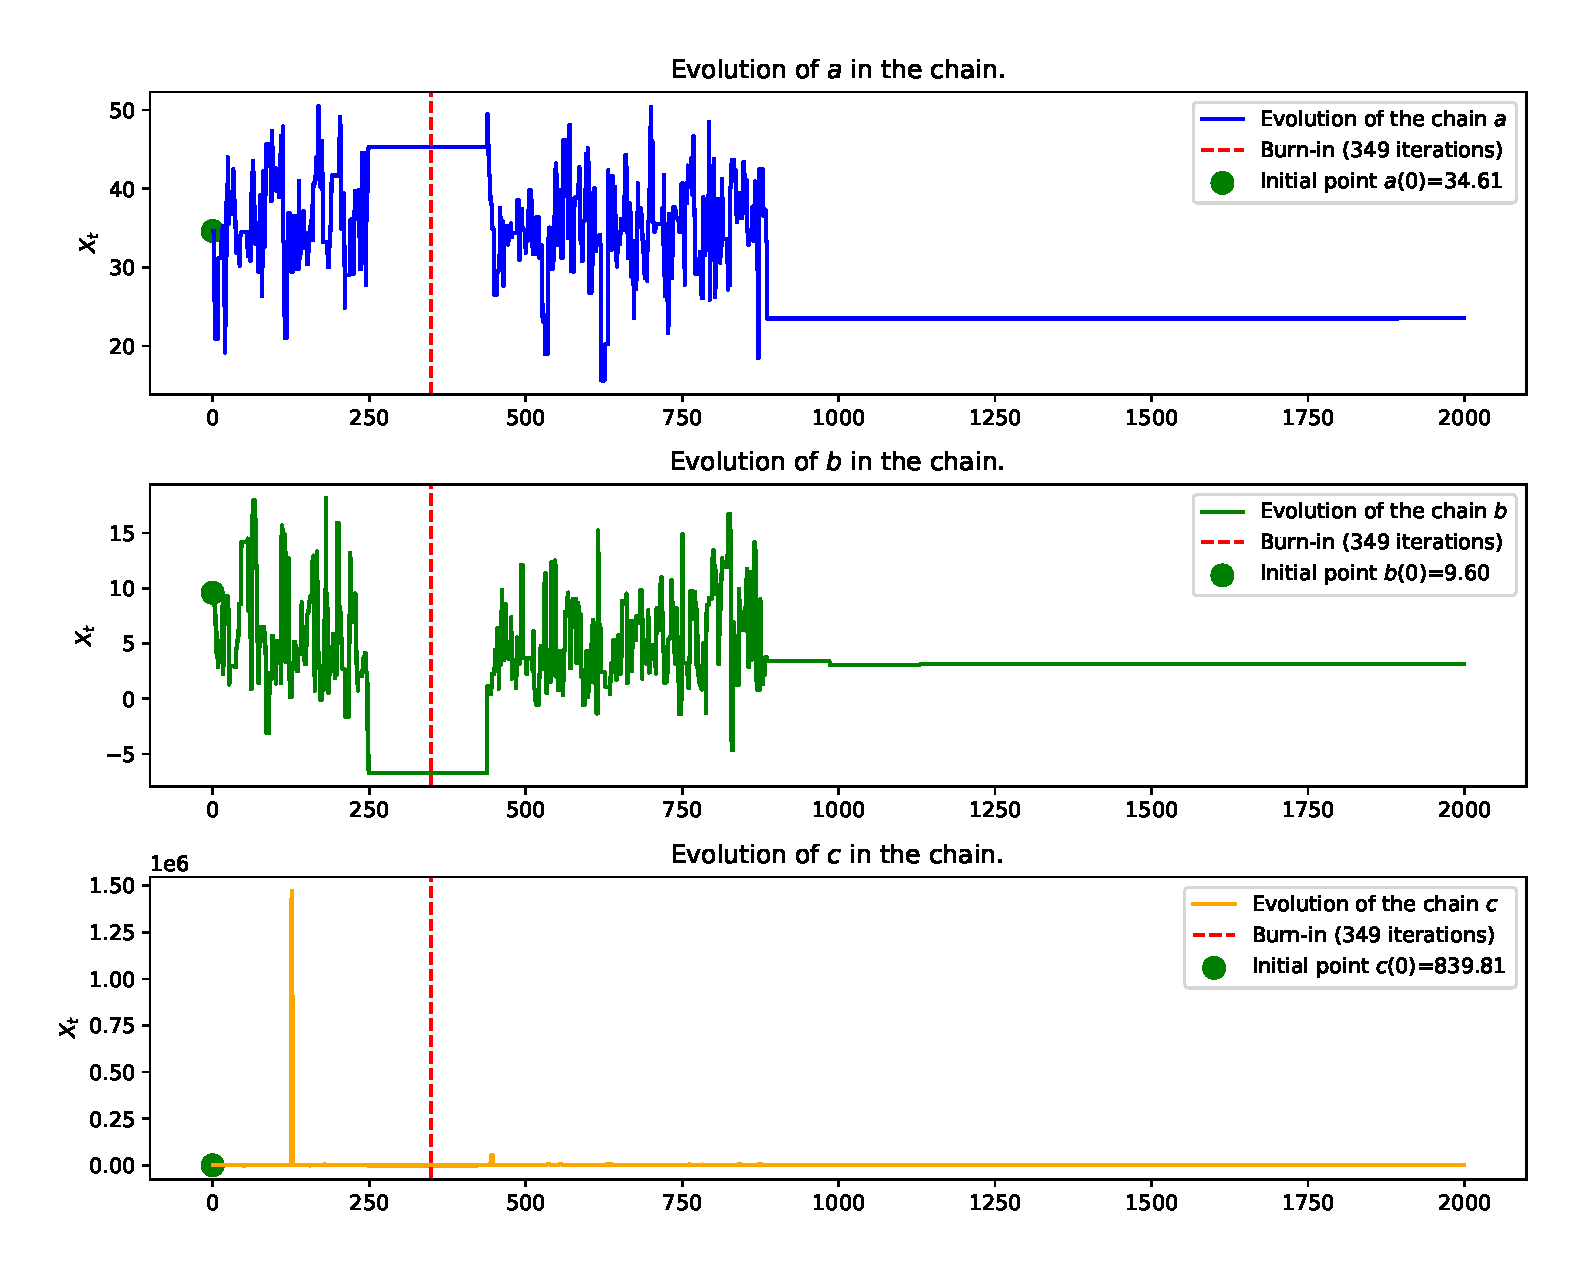
\includegraphics[width=0.845\textwidth]{IMAGENES/marginal_evolution_ex2.pdf}
\end{figure}

También se tiene la trayectoria de la cadena de Markov en el espacio de parámetros para cada par de parámetros.

\begin{figure}[h!]
	\centering
	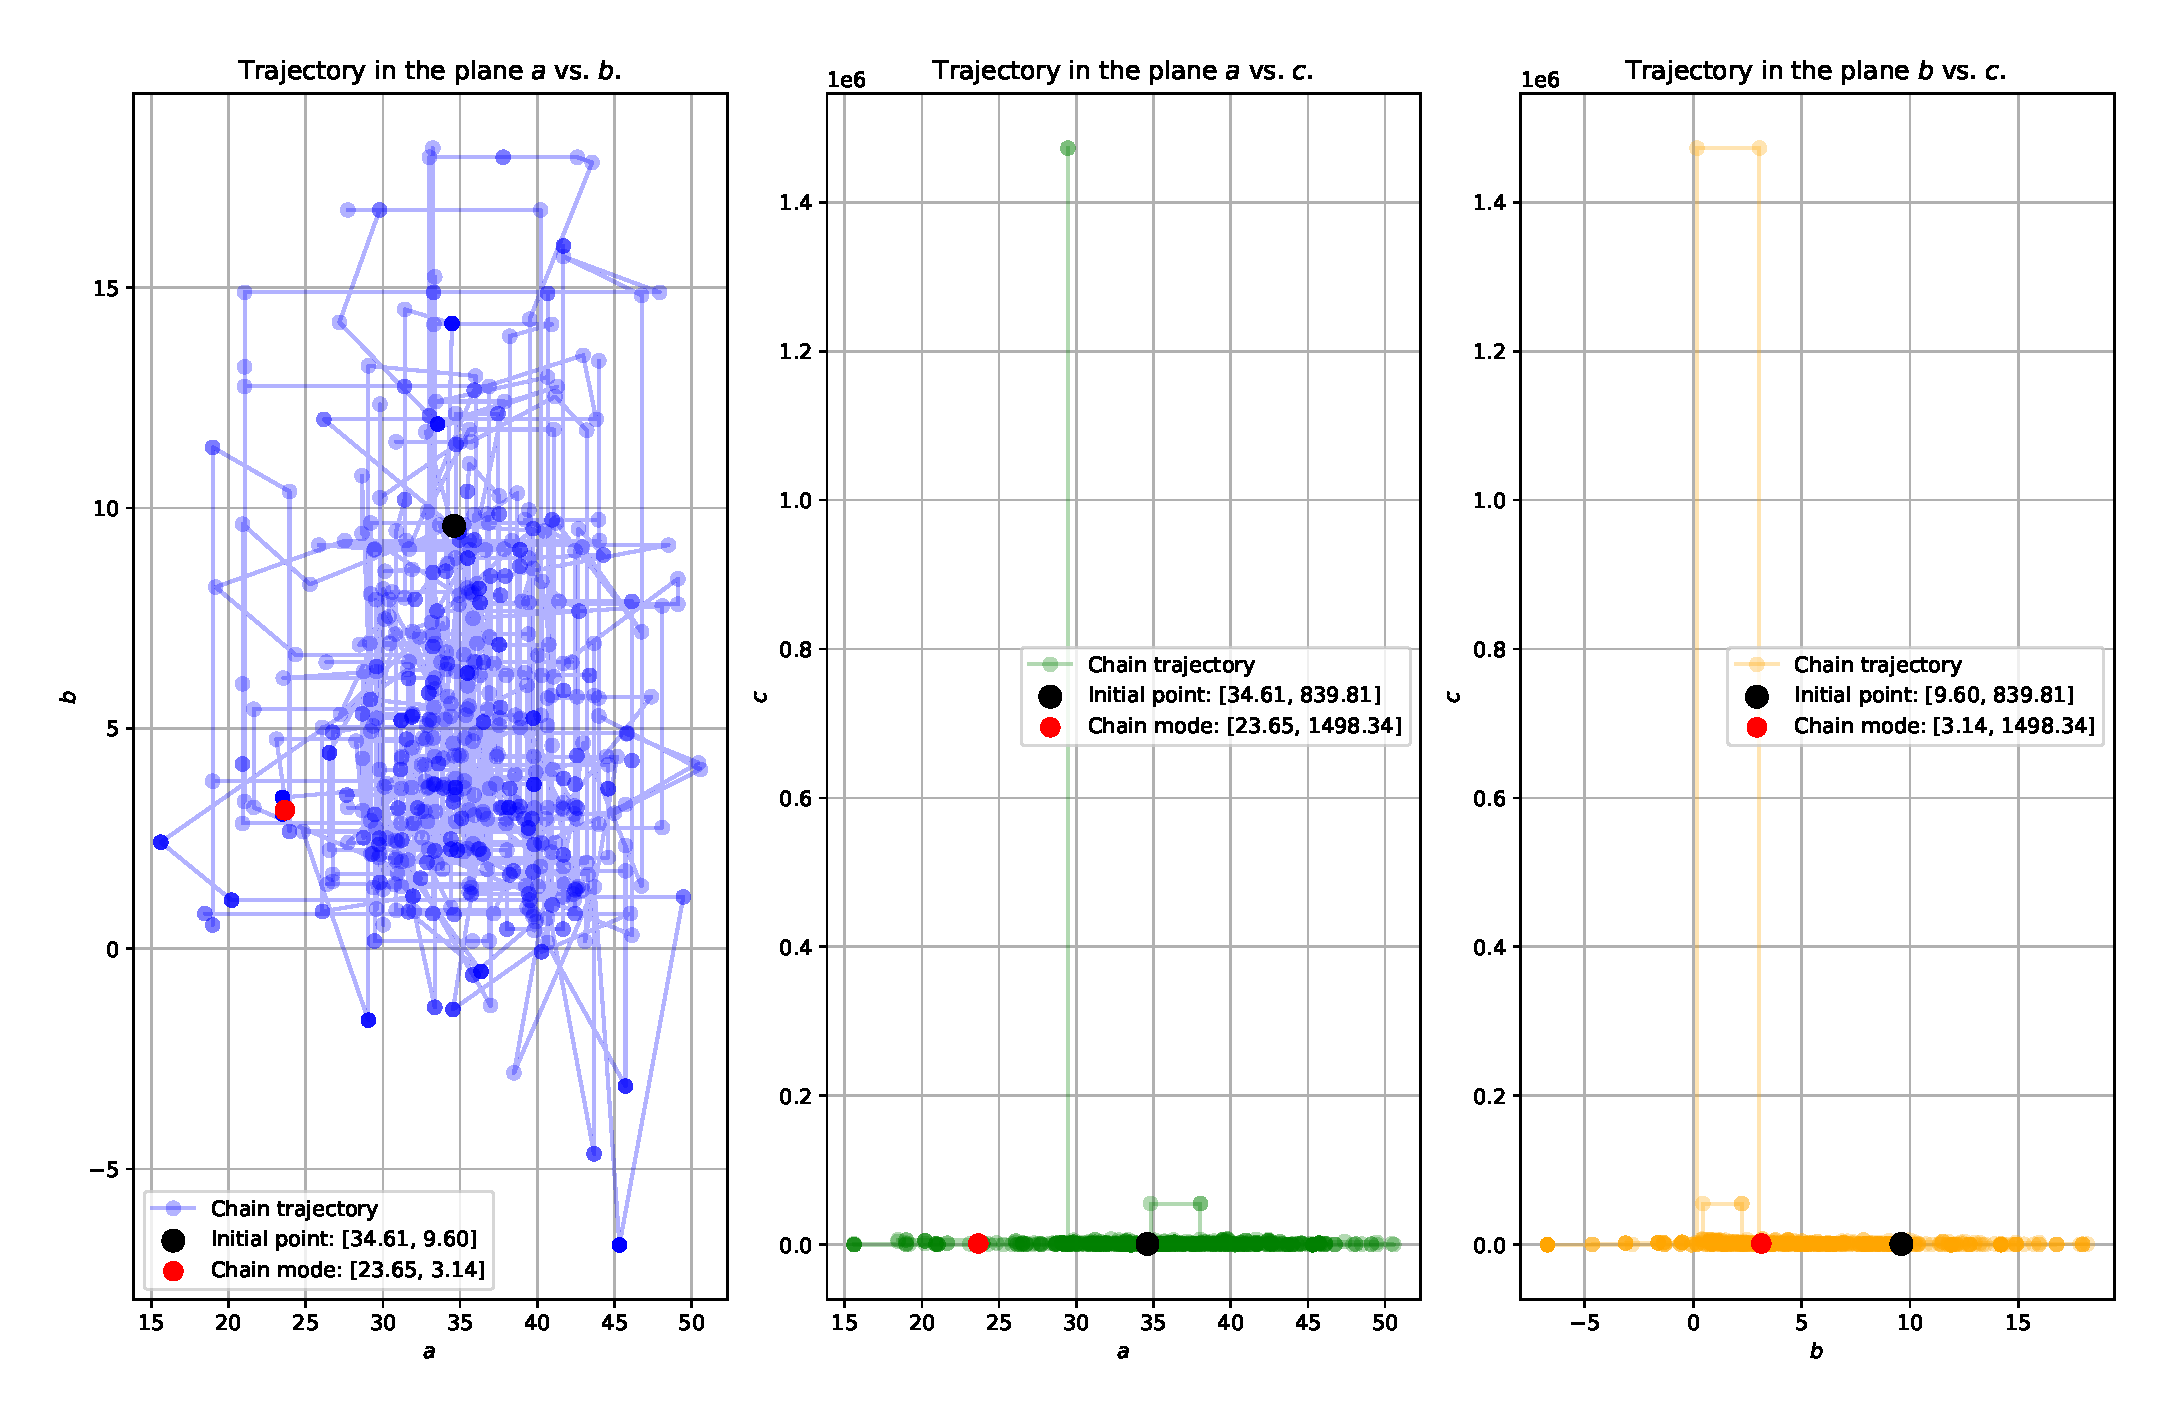
\includegraphics[width=0.845\textwidth]{IMAGENES/trayectory_ex2.pdf}
\end{figure}

Antes de incluir la propuesta Gibbs para $c$, todos estos gráficos resultaban con mucha variabilidad y sin convergencia clara. Ahora, se puede ver la convergencia rápida de $c$. Finalmente, se tiene el gráfico de los datos iniciales comparado con las estimaciones de $\lambda_{i}$. Podemos notar que se ajusta muy bien. Este resultado suele ser recurrente en la experimentación, sin embargo, se notó una mejora importante con la inclusión de la propuesta Gibbs para $c$.
\begin{figure}[h!]
	\centering
	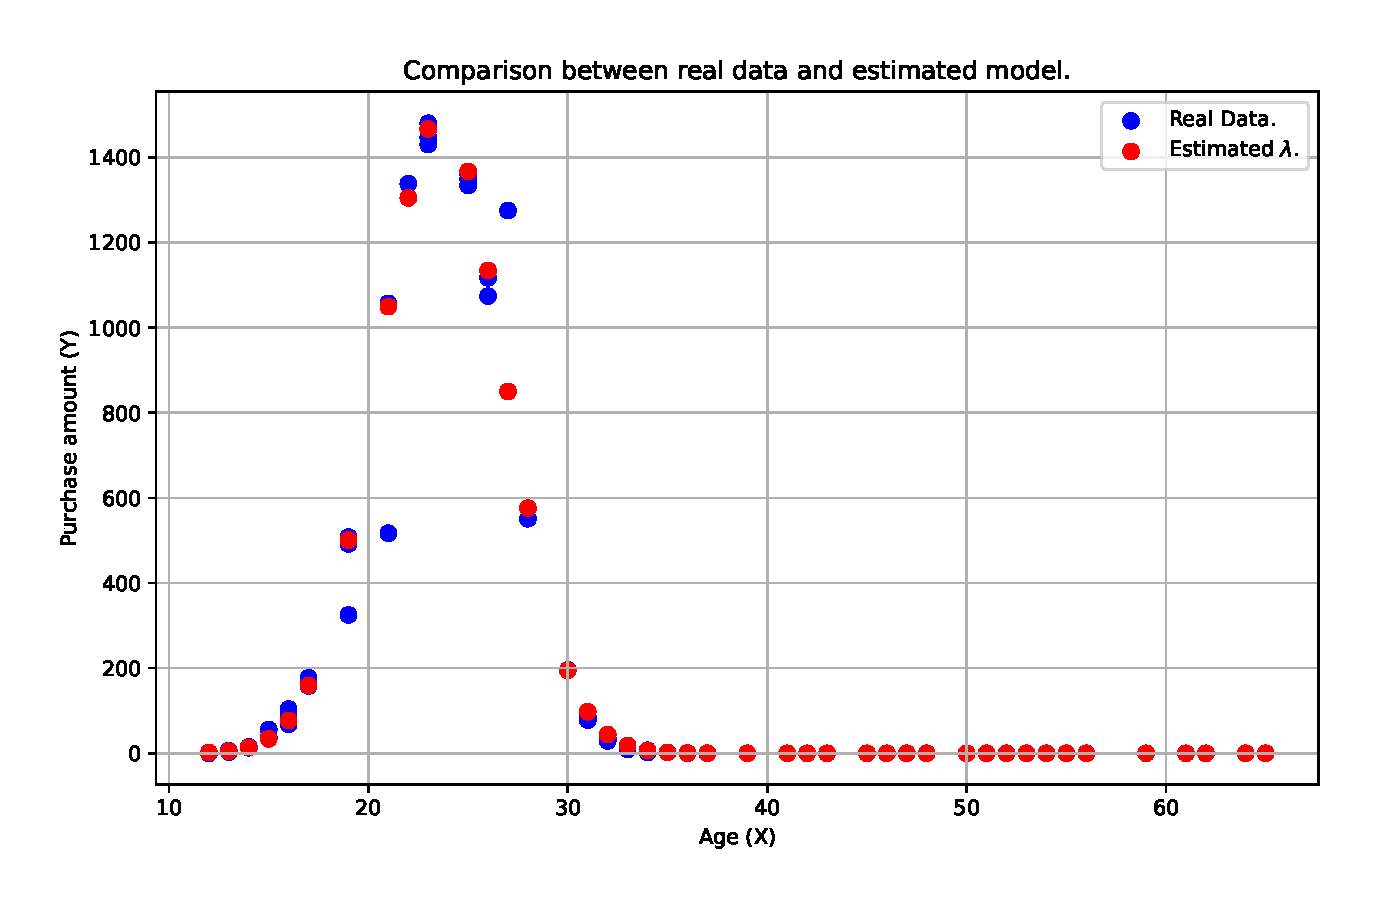
\includegraphics[width=0.845\textwidth]{IMAGENES/comparision_ex2.pdf}
\end{figure}